\documentclass{article}[12pt]
\usepackage{physics}
\usepackage{setspace}
\usepackage{amsmath}
\usepackage{mathrsfs}
\usepackage{amssymb}
\usepackage{feynmp-auto}
\usepackage{tgtermes}
\usepackage{graphicx}
\usepackage{booktabs}
\usepackage{array}
\usepackage{caption}
\usepackage{listings}
\usepackage{xcolor}
\usepackage{helvet}
\definecolor{codegreen}{rgb}{0,0.6,0}
\definecolor{codegray}{rgb}{0.5,0.5,0.5}
\definecolor{codepurple}{rgb}{0.58,0,0.82}
\definecolor{backcolour}{rgb}{0.95,0.95,0.92}
\definecolor{lightgray}{rgb}{0.95,0.95,0.95}

\lstdefinestyle{mystyle}{
    backgroundcolor=\color{lightgray},   
    commentstyle=\color{codegreen},
    keywordstyle=\color{magenta},
    numberstyle=\tiny\color{codegray},
    stringstyle=\color{codepurple},
    basicstyle=\fontfamily{pcr}\selectfont\footnotesize,
    breakatwhitespace=false,         
    breaklines=true,                 
    captionpos=b,                    
    keepspaces=true,                 
    numbers=left,                    
    numbersep=5pt,                  
    showspaces=false,                
    showstringspaces=false,
    showtabs=false,                  
    tabsize=2
}
\numberwithin{equation}{section}
\lstset{style=mystyle}
\captionsetup{font=footnotesize}
\newcommand{\RN}[1]{%s
  \textup{\uppercase\expandafter{\romannumeral#1}}%
}
\setcounter{section}{2}
\setcounter{page}{23}
\setcounter{figure}{10}
\usepackage{geometry}
\geometry{
 a4paper,
 left=25.4mm,
 right=25.4mm,
 top=30mm,
 bottom=25.4mm
 }
\begin{document}
\section{Numerical calculation for integro-differential equation}

\begin{spacing}{1.5}
The integro-differential equation central to the analysis of our model was solved numerically using C++ code.  This section outlines the key computational techniques employed within the code.

\subsection{4.1 Structure of C++ code}
The structure of the C++ code designed to solve the integro-differential equation is outlined below. 
The C++ code for solving the integro-differential equation is structured as follows: the functions performing the calculations are declared beforehand within a header file (.hpp) using a class, and then defined within a source file (.cpp).
Appropriate numerical methods were adopted for each computational step.
$\\$
\begin{figure}[htbp]
  \centerline{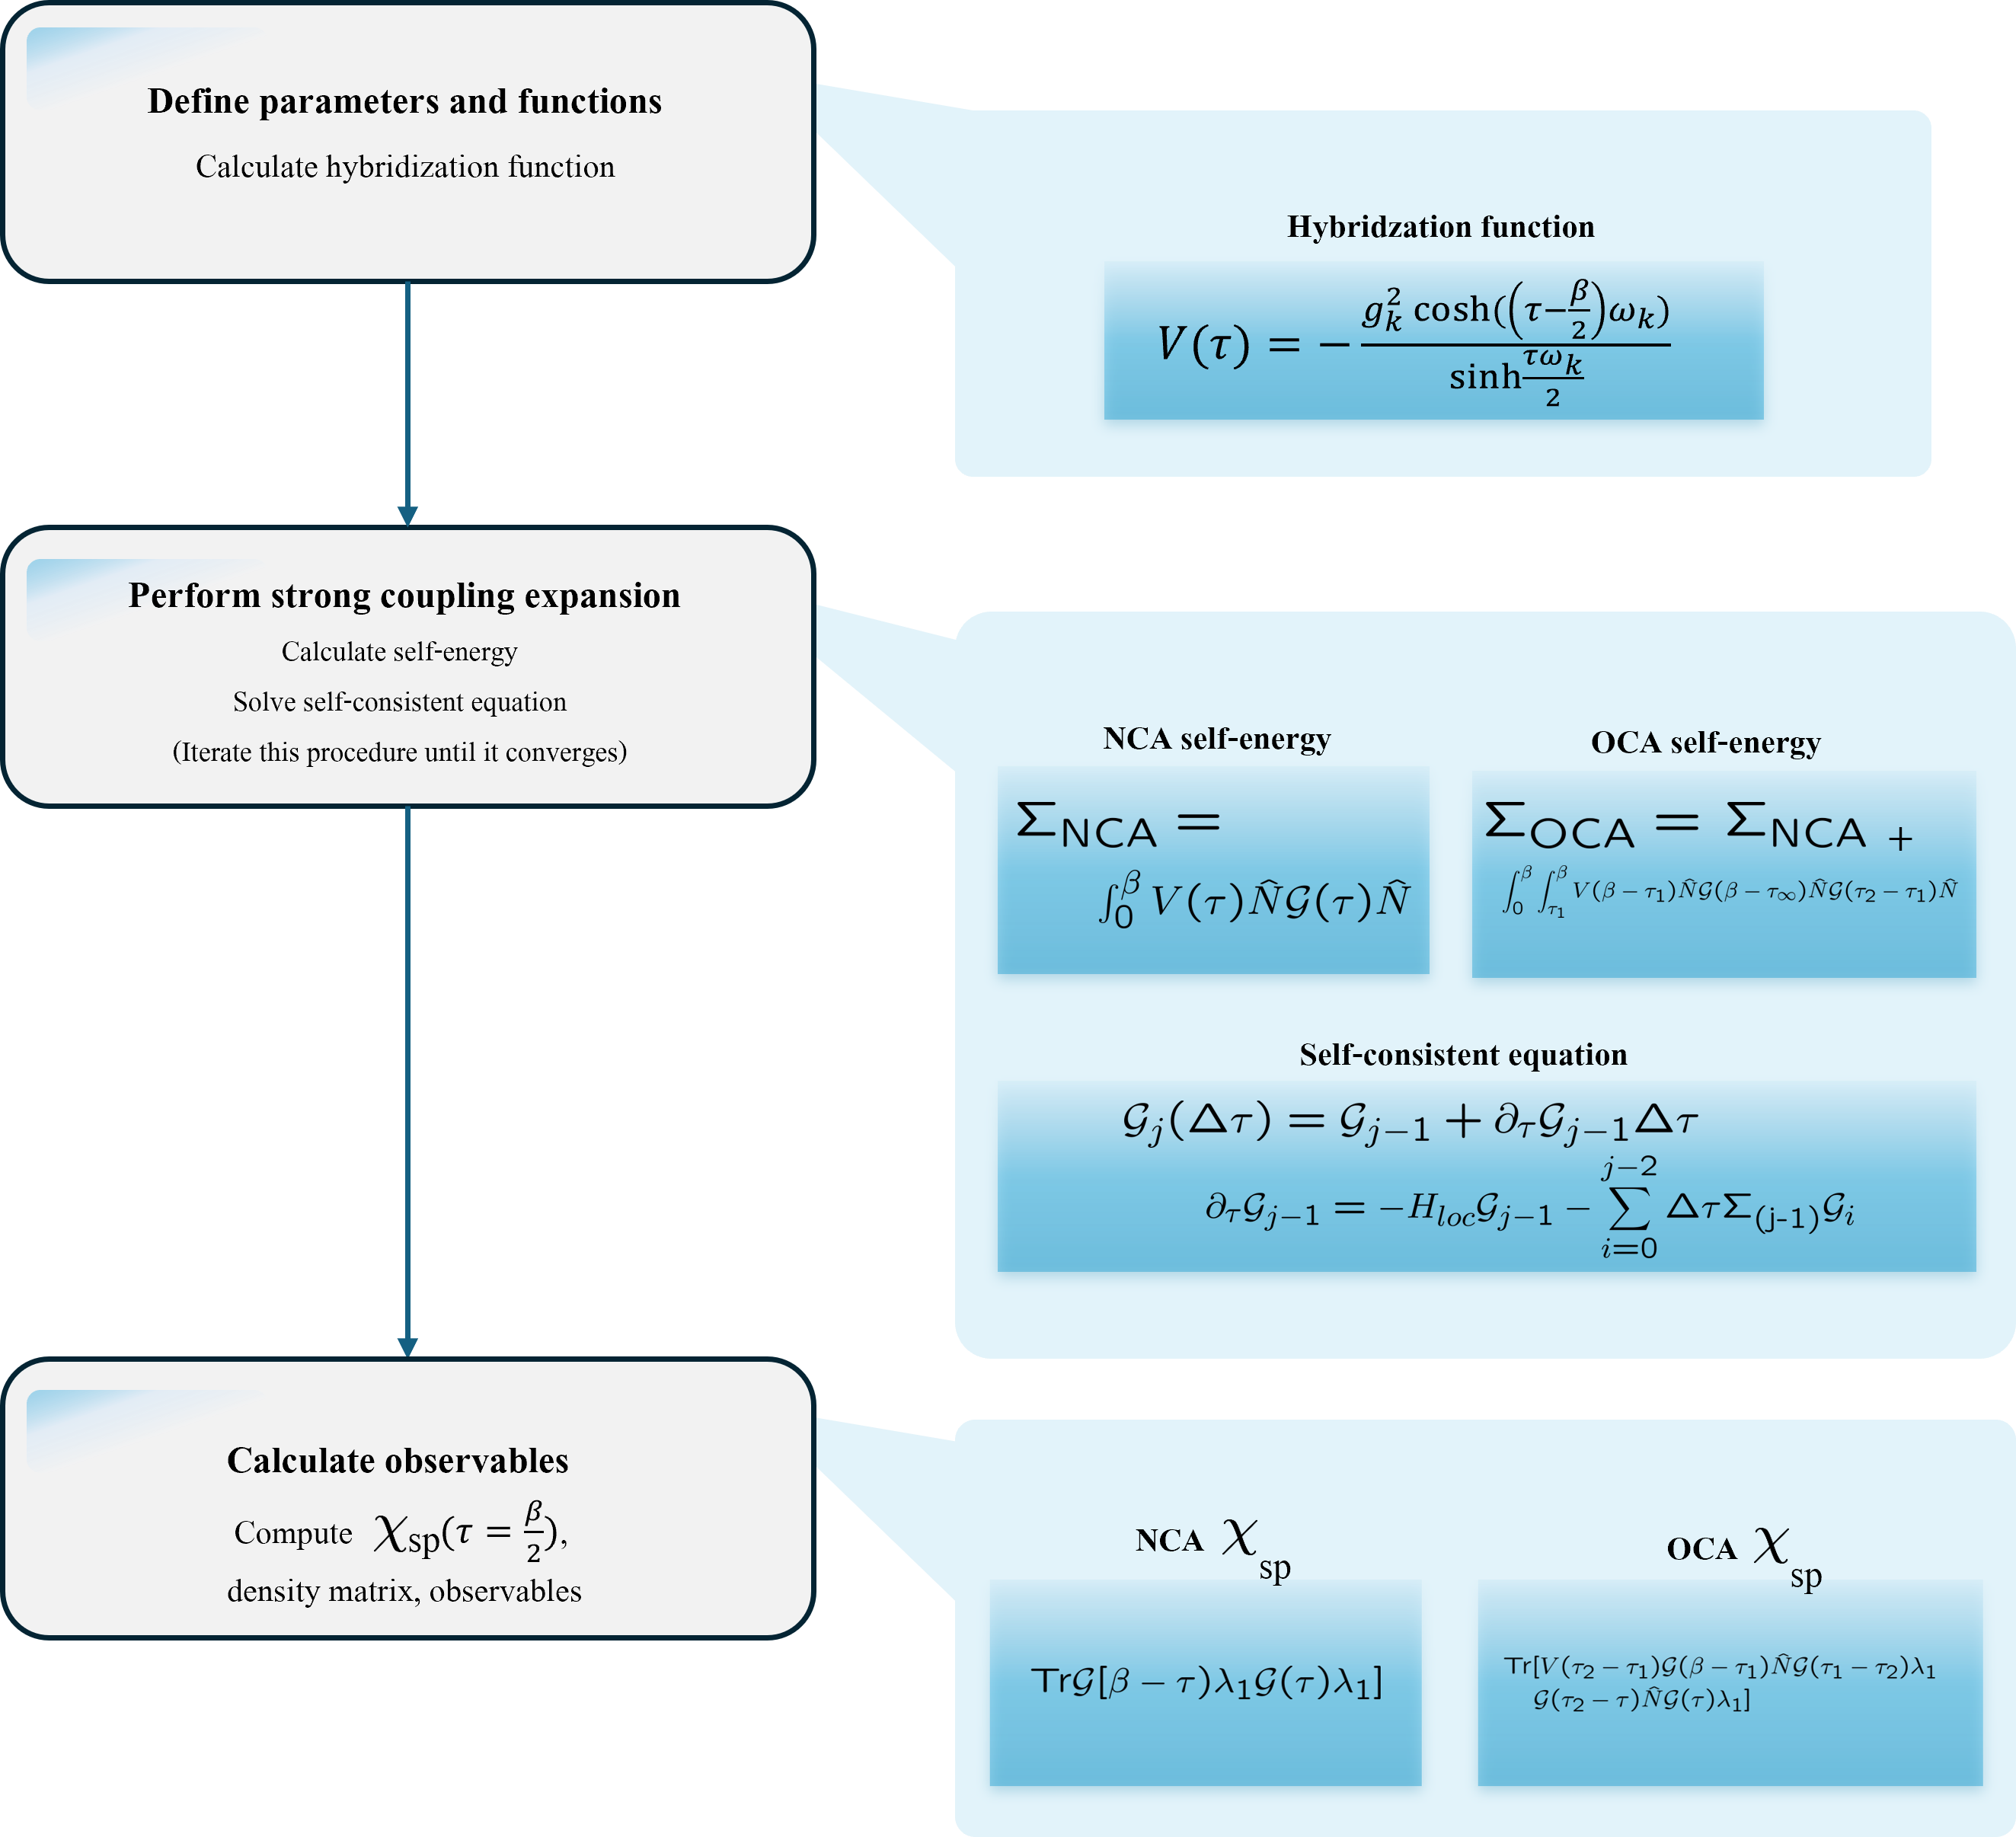
\includegraphics[width=13cm]{TexFigure/Flowchart_brokengraph.png}}
  \caption{The flowchart of Program structure}
\end{figure}

\subsection{4.2 Hybridzation function - Simpson’s Rule}
The hybridization function, calculated as a scalar rather than a matrix, was evaluated by considering the form of the retarded Matsubara Green's function. To compute the value of $g_k$, a parameter that determines the coupling between the RC circuit and the Josephson junction, Simpson's rule of integration was employed. The formula for calculating $g_k$ for the application of this integration method is given below:
\begin{flalign}
g_k =\sqrt{\frac{2W}{\alpha}\bigg(\frac{W}{1+(\nu x)^2}\bigg)} \qquad, \quad (x=\frac{k}{W})
\end{flalign}
The integration method using Simpson’s method follows:
\begin{flalign}
\int f(x) dx = \frac{b-a}{3n} \bigg[f(x_0) + \sum_{i=odd} 4f(x_i) + 2\sum_{i=\text{even}}f(x_i)+f(x_0) + f(x_f)\bigg]
\end{flalign}
Here, we calculate the initial value using the case of $V(\tau,k=0)$. 
The part where the Simpson's rule is implemented in the code is as follows. After generating a vector array suitable for the length of the k-index to calculate  V(τ),  the integration is performed only for the k-value for $g_k$ and $\omega_k$ in the V(τ) expression. Using the resulting expression, the value for each τ interval is stored in an array of length τ.

\subsection{4.3 Trapezoidal method}
The trapezoidal method was employed for the calculation of the self-energy and the propagator. This section provides a brief overview of the implementation for calculating the propagator. The numerical integration formula using the trapezoidal method is as follows: 

\begin{flalign}
\int_{a}^{b} f(x) \, dx \approx \frac{\Delta x}{2} \left[ f(x_0) + 2f(x_1) + 2f(x_2) + \dots + 2f(x_{n-1}) + f(x_n) \right]
\end{flalign}

To correspond to the actual numerical integration program code, the formula can be rewritten in the form of an infinite series as follows:
\begin{flalign}
\int_{a}^{b} f(x) \, dx \approx \Delta x \left[ \frac{1}{2}f(x_0) + \sum_{j=1}^{n-1} f(x_j) +  \frac{1}{2}f(x_n) \right]
\end{flalign}
And the self-consistent equation we aim to solve is as follows:
\begin{flalign}
\mathcal{G}_j = \mathcal{G}_{j-1}+\partial_\tau\mathcal{G}_{j-1}\Delta\tau
\end{flalign}
When implementing the trapezoidal method, it's crucial to follow a specific sequence of calculations:

1. First, update the value of $\partial_\tau\mathcal{G}_i$ using $\mathcal{G}_i$, which corresponds to each $f(x_i)$.

2. Next, calculate the temporary value of $\mathcal{G}'_{i+1}$ using the updated $\partial_\tau\mathcal{G}_i$.

3. Then, calculate $\partial_\tau\mathcal{G}_{i+1}$using the temporary value of $\mathcal{G}'_{i+1}$ calculated in the previous step.

4. Finally, perform the final trapezoidal integration calculation using $\frac{1}{2}(\partial_\tau\mathcal{G}_i + \partial_\tau\mathcal{G}_{i+1})$.
$\\$To implement this in the program, we introduced two arrays: P-array to store the final calculation result $\mathcal{G}_i$, 
and S-array to store the temporary value calculated in step 2. We also devised a method to use the value of S-array in step 3.
This process is visually represented in the diagram below, where:
\begin{figure}[htbp]
  \centerline{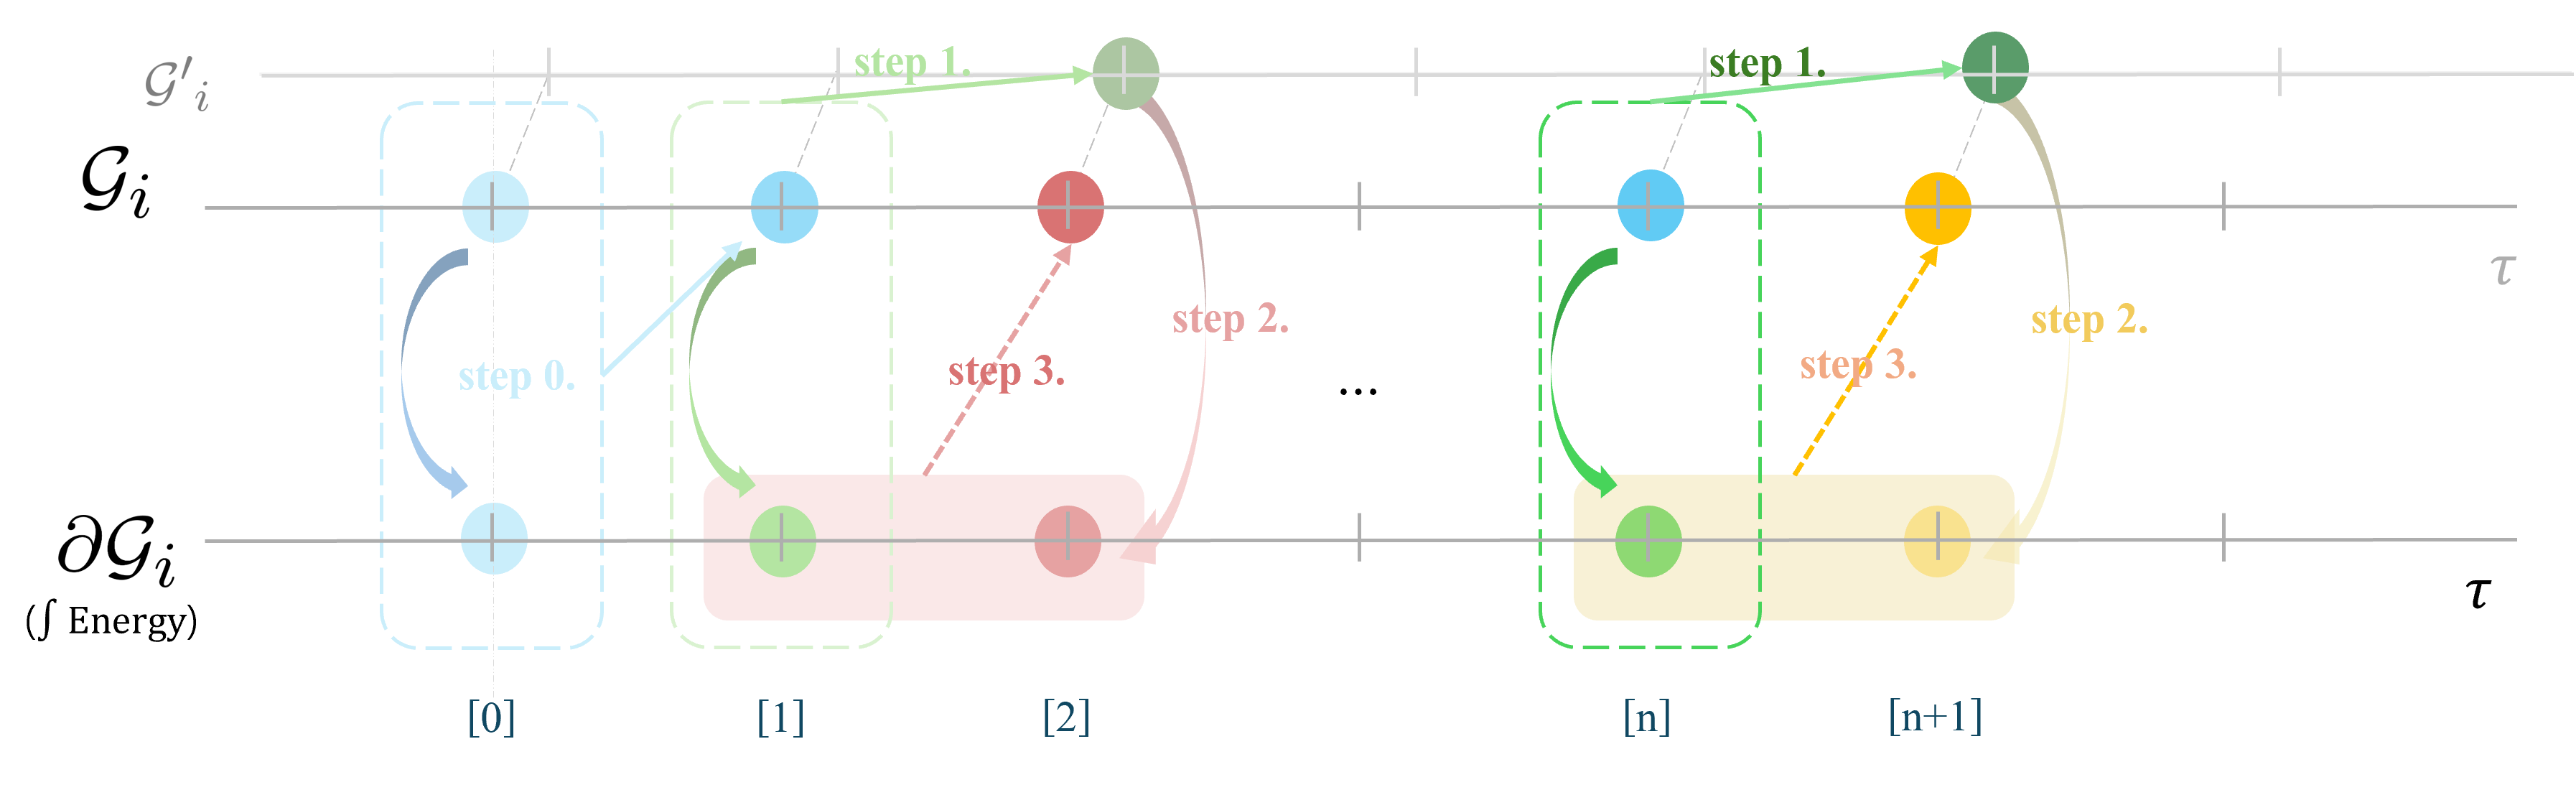
\includegraphics[width=15cm]{TexFigure/self_structure.png}}
  \caption{Image depicting the procedure of Trapezoidal process}
\end{figure}

This is implemented in the code as follows:
\begin{lstlisting}[language=C++, caption=Trapezoidal calculation code]
vector<MatrixXd> MD_OC::Propagator(const vector<MatrixXd>& sig, const MatrixXd& loc)
{
    vector<MatrixXd> P_arr(t, MatrixXd::Zero(siz,siz)); // Declaration of an array to store the final calculation result
    vector<MatrixXd> S_arr(t, MatrixXd::Zero(siz,siz)); // Declaration of an array to store temporary results during calculation
		
    P_arr[0] = MatrixXd::Identity(siz,siz);
    S_arr[0] = MatrixXd::Identity(siz,siz);

    MatrixXd sig_form = MatrixXd::Zero(siz,siz); // A matrix to temporarily store the result of process 1.
    MatrixXd sig_late = MatrixXd::Zero(siz,siz); // A matrix to temporarily store the result of process 3.


    for (int i = 1; i < t; i++)
    {
        P_arr[1] = P_arr[0];
        sig_late = 0.5 * Delta_t * (0.5 * Delta_t * (sig[1] * P_arr[0] + sig[0] * (P_arr[0] + Delta_t * P_arr[0])));
        P_arr[1] = P_arr[0] - 0.5 * Delta_t * loc * (2 * P_arr[0] + Delta_t * P_arr[0]) + sig_late;
        S_arr[1] = P_arr[1];

        if (i > 1)
        {
            sig_form = round_propagator_ite(loc, sig, P_arr, i - 1, 0);
            S_arr[i] = P_arr[i - 1] + Delta_t * sig_form; // Calculation process of 2. is performed in this part.

            sig_late = 0.5 * Delta_t * (round_propagator_ite(loc, sig, P_arr, i - 1, 1) + round_propagator_ite(loc, sig, S_arr, i, 1)); // This part is the result of performing trapezoidal calculation for the integral calculation in the round propagator.
            P_arr[i] = P_arr[i - 1] - 0.5 * Delta_t * loc * (2 * P_arr[i - 1] + Delta_t * sig_form) + sig_late; // This part is the result of performing trapezoidal calculation for the integral calculation in the round propagator.

        }
    }

    return P_arr;
}
\end{lstlisting}
\subsection{4.4 Iteration truncation - Relative entropy}

The integro-differential equation we target to solve has a recursive structure, which means that a single calculation is not enough to get a complete result. The obtained array of $G(\tau)$ in the previous iteration is to be used as an initial condition for multiple iterative calculations until the result converges sufficiently. To truncate the iteration of calculations in flexibility, the concept of relative entropy was introduced into the code. The formula for calculating relative entropy is as follows:
\begin{equation*}
D(p||q) = \sum_{x\in\mathcal{X}}p(x)\ln\frac{p(x)}{q(x)}
\end{equation*}
In the case of $\mathcal{G}(\tau = \beta)$ in the interval $[0,\beta]$, The Green's function is represented by the same formula as the partition function of a thermal equilibrium state in the grand canonical ensemble. In this case, the partition function plays the same role as the density operator, which represents the mixed state of the system being investigated from a quantum mechanical perspective.
In quantum mechanics, each diagonal element of the density operator represents the probability of observing the corresponding energy level in the system. This allows us to calculate the probability distribution in the final stage. The code was designed to terminate the calculation of G(τ) when the distance between the probability distributions obtained at each calculation step becomes sufficiently small, indicating that the result has converged.

\begin{lstlisting}[language=C++, caption=Iteration truncation code]
// Function that returns the value of \mathcal{G}(\tau=\beta)
vector<double> MD_OC::temp_itemin(vector<MatrixXd> &arrr, double minpo, int size)
{
    vector<double> dist_return(size,0);
    for (int i = 0 ; i < size; i++){
        dist_return[i] = arrr[t-1](i,i); // Value of \mathcal{G} at \tau = \beta
    }
    return dist_return;
}

// Function that processes recursive calculation.
vector<MatrixXd> MD_OC::Iteration(const int& n)
{
    // ~ Calculation part
    //////////////////////////////////////////////////////////////
    double temp_minpoin;
    vector<vector<double> > temp_itemi(2,vector<double>(siz,0)); // Arrays to store the results of the previous and current iteration. siz represents the dimension of the calculated square matrix.
    double RELA_ENTROPY;
    ///////////////////////////////////////////////////////////////
    
    for (int i = 0; i <= n; i++){
        // ~ Calculation part
            //////////////////////////////////////////////////////////////////////////////

            temp_minpoin = //beta value; 

            //////////////////////////////////////////////////////////////////////////////
       // ~ Calculation part
           /////////////////////////////////////////////////////////////////////////////

            temp_itemi[(i-1)%2] = temp_itemin(Prop,temp_minpoin,siz); // temporary store previous iteration data
            RELA_ENTROPY = 0;

            ////////////////////////////////////////////////////////////////////////////
      // ~ Calculation part
            /////////////////////////////////////////////////////////////////////////////

            temp_itemi[i%2] = temp_itemin(Prop,temp_minpoin,siz); // temporary store present iteration data
            
            // Relative entropy calculation
            
            for (int j = 0; j < siz; j++){
                RELA_ENTROPY += temp_itemi[i%2][j] * log(temp_itemi[i%2][j]/temp_itemi[(i-1)%2][j]);
            }
            

            if (i > 1){
                cout << "\t""\t" << i << " th Iteration stop value : " << fabs(RELA_ENTROPY) << endl;
                if (fabs(RELA_ENTROPY) < 0.00001){
                    break; // If the distance between the probability distributions of the previous and current steps is less than 0.00001, the calculation is terminated.
                } 
            }
            /////////////////////////////////////////////////////////////////////////////
        }
    return //(Calculation result);
}
\end{lstlisting}
\subsection{4.5 Implementation of T-matrix}
The T-matrix was first introduced in the process of representing the OCA self-energy formula in diagrammatic form. Implementing this in a computational setting leads to a reduction in the calculation time of the approximation method. The basic idea is to pre-calculate the product of the propagator and the N matrix, store it in matrix form, and then use the values from the matrix elements as needed during the self-energy calculation.

\subsubsection*{Correlation function calculation}
Inspired by the T-matrix approach, a similar method was adopted for calculating the correlation function,$\chi_{sp}$. In the case of OCA, a total of 8 matrix multiplications are required, and considering the array indices, the calculation process occurs 4 times. This can be simply represented as follows:
\begin{flalign}
\chi_{sp} = V_{mn}\text{Tr}(\hat{\mathcal{G}}_{k-m-1}*\hat{N}*\hat{\mathcal{G}}_{m-i}*\hat{\lambda}_1*\hat{\mathcal{G}}_{i-n}*\hat{N}*\hat{\mathcal{G}}_{n}*\hat{\lambda}_1)
\end{flalign}
If the part corresponding to $\hat{N} * \hat{\mathcal{G}_i}*\hat{N}*\hat{\mathcal{G}_j}*\hat{\lambda}_1$ is pre-computed and stored in matrix form for later use in the calculation, the eight matrix multiplications are reduced to a single matrix multiplication.
\begin{flalign}
\hat{T}_{chi} =\hat{\mathcal{G}}_{i'}*\hat{N}*\hat{\mathcal{G}}_{j'}*\hat{\lambda}_1\\ \chi_{sp} = \text{Tr}( \hat{T}_{chi} * \hat{T}_{chi}')
\end{flalign}
\subsubsection*{$\chi_{sp}$ T-matrix $\hat{T}_{chi}$ : k=3 case}
The code for the general formula to calculate  $\chi_{sp}$ before introducing the T-matrix is as follows:
\begin{lstlisting}[language=C++, caption=Full One-crossing Approximation implementation code]
for (int i=0; i<k; i++)
{
	  MatrixXd Stmp = MatrixXd::Zero(3,3);
			for (int n=0; n<=i; n++) for (int m=i; m<k; m++)
      {
         Stmp += V[m-n] * Prop[k-m-1] * N * Prop[m-i] * GELL 
					         * Prop[i-n] * N * Prop[n] * GELL;
      }
      OCA_chi_array0[i] = pow(Delta_t,2)*Stmp.trace();
}
\end{lstlisting}
In the above equation, for the case of k=3, the number of calculation cases according to n, m, and i is as follows:
\begin{figure}[htbp]
  \centerline{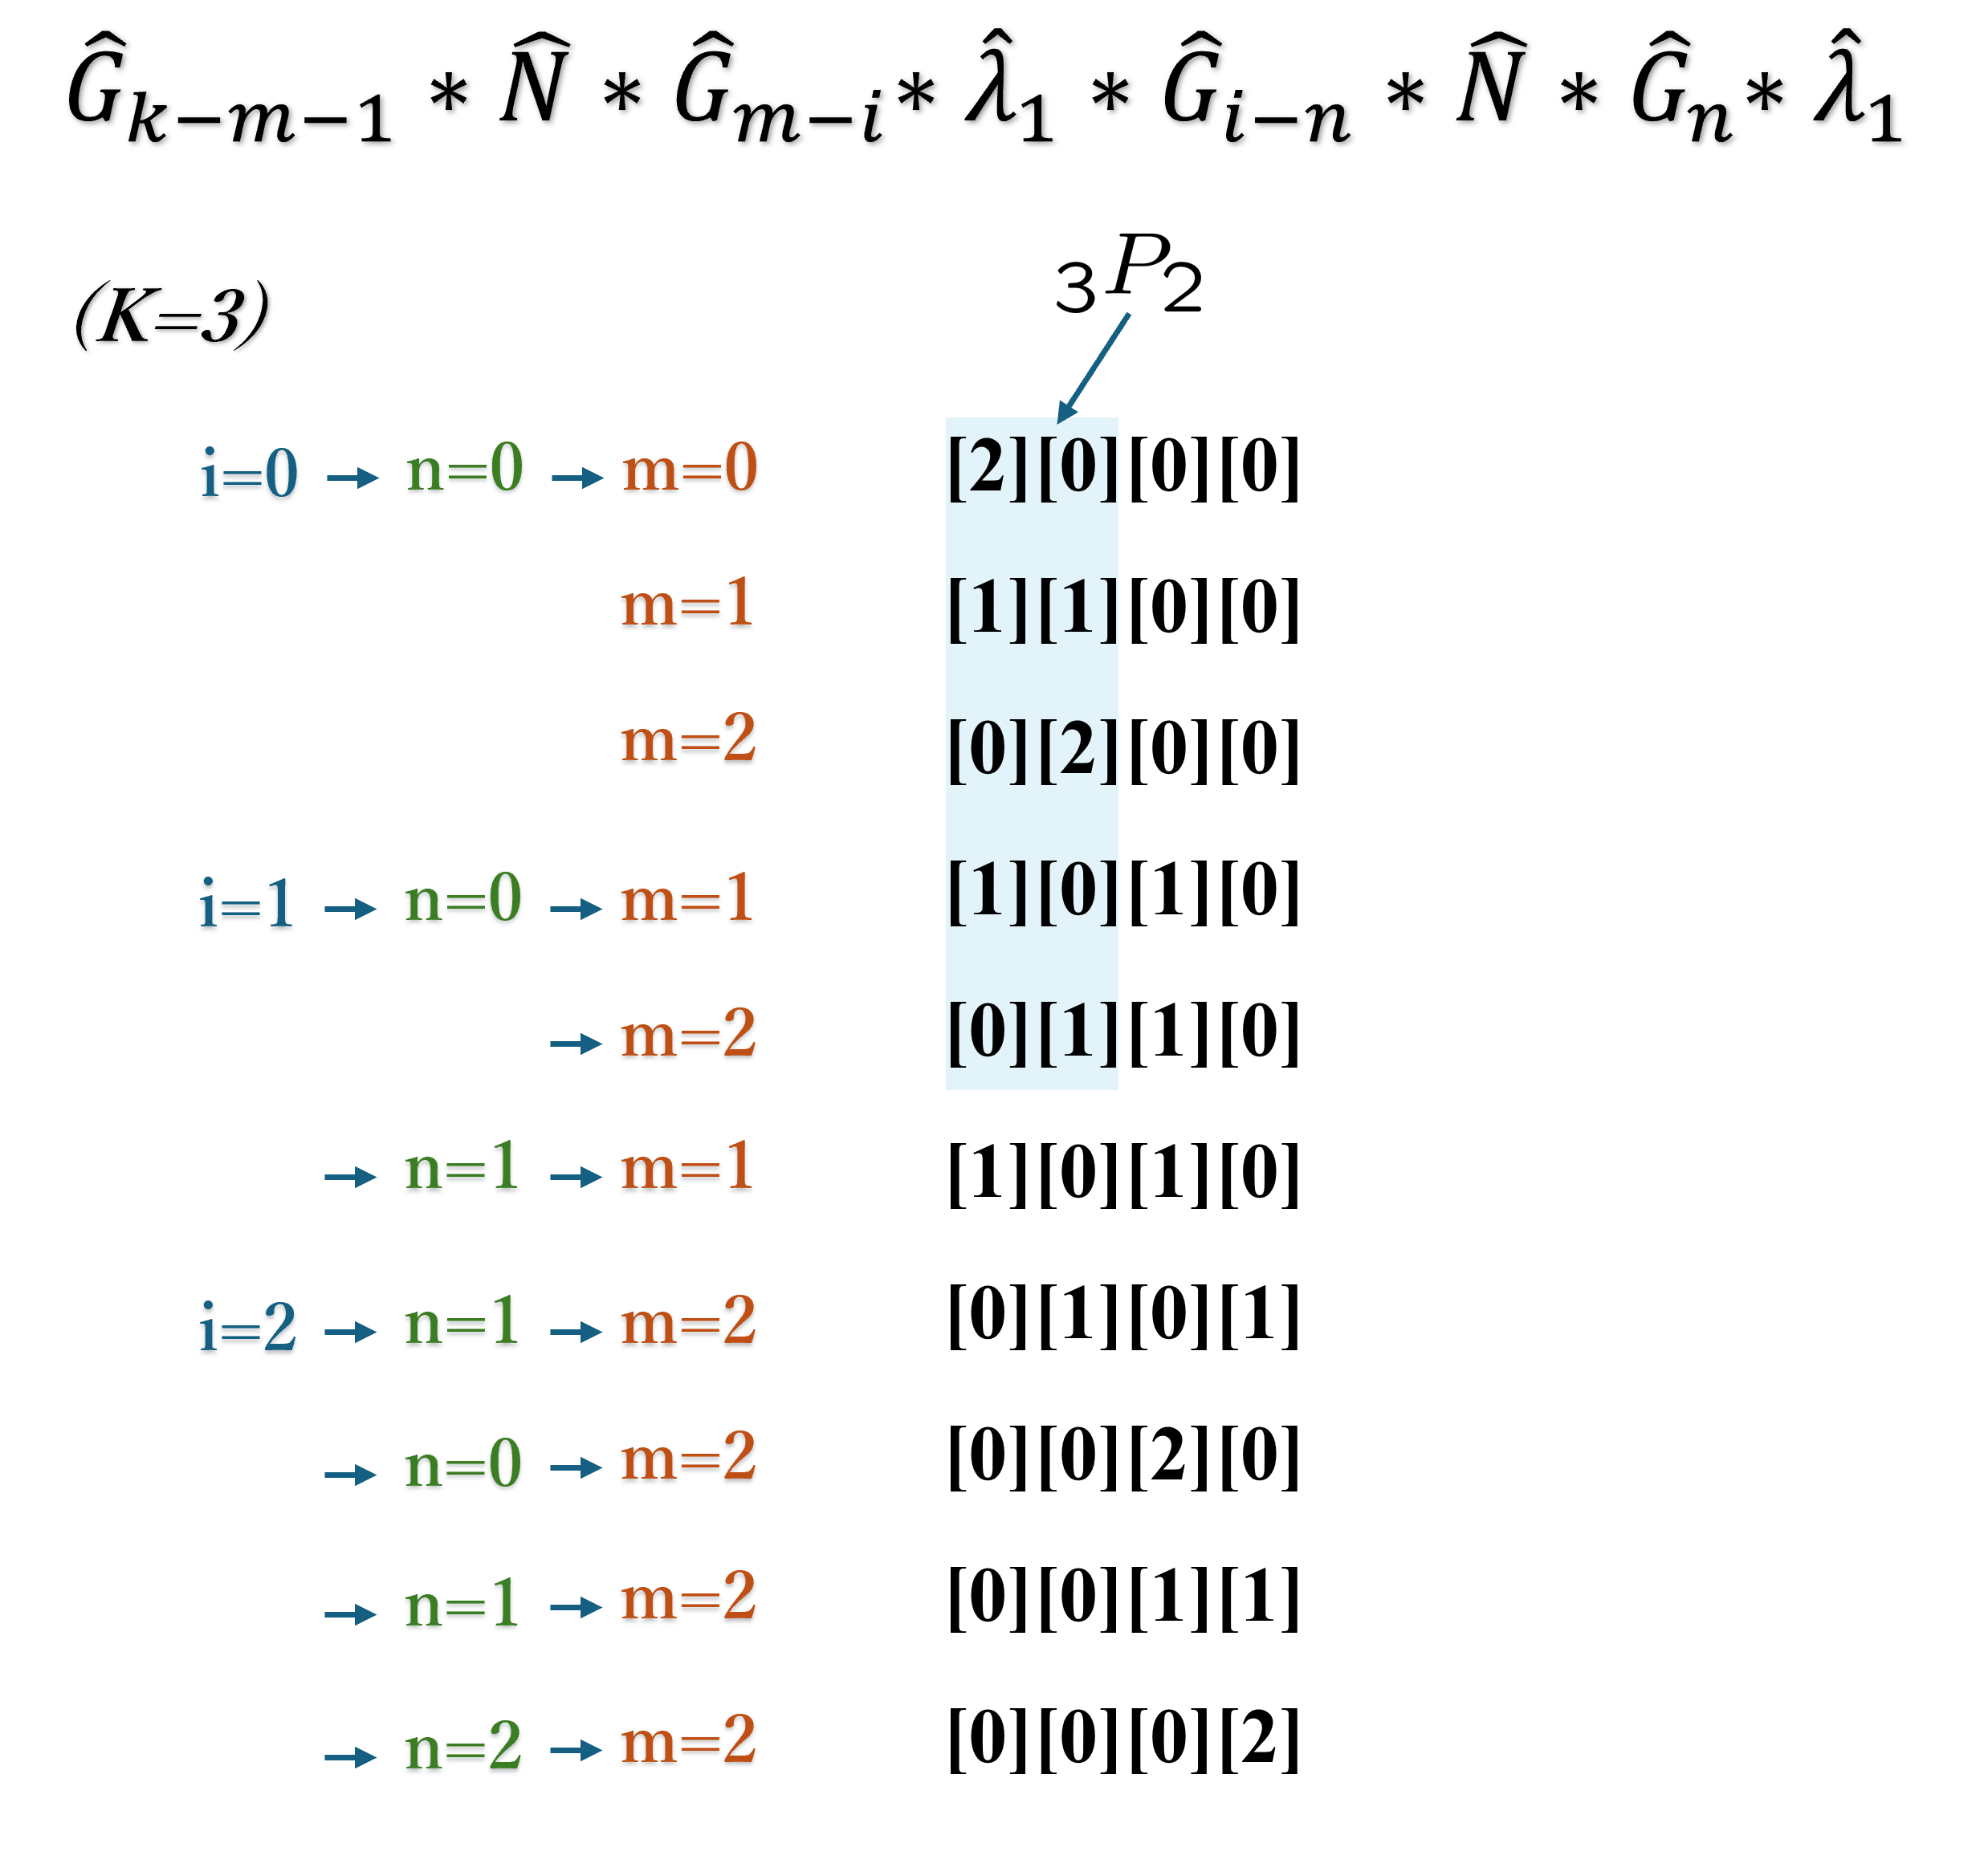
\includegraphics[width=12cm]{TexFigure/Tmat.png}}
  \caption{Possible calculation cases in k=3}
\end{figure}
Here, we can see that the total number of calculation cases can be represented by selecting and arranging two numbers from the three numbers 2, 1, and 0. To achieve this, we can introduce the following matrix:
\begin{figure}[htbp]
  \centerline{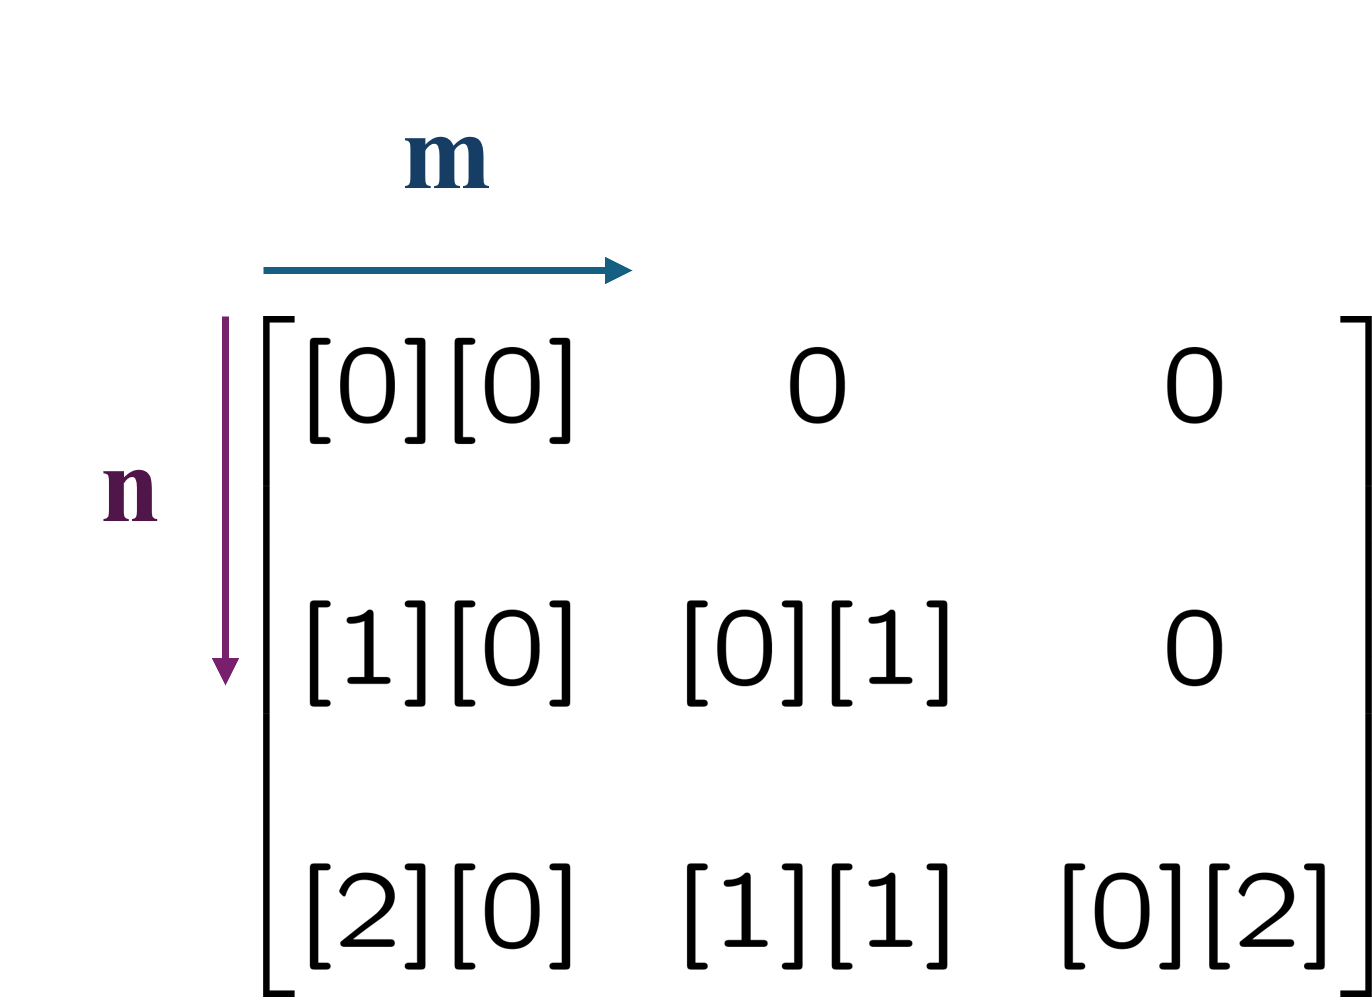
\includegraphics[width=9cm]{TexFigure/Tmat2.png}}
  \caption{The Structure of correlation-matrix}
\end{figure}
For example, if we want to represent all the possible cases as shown above, using the matrix above and calculating as below, we obtain all possible calculation cases.
\begin{figure}[htbp]
  \centerline{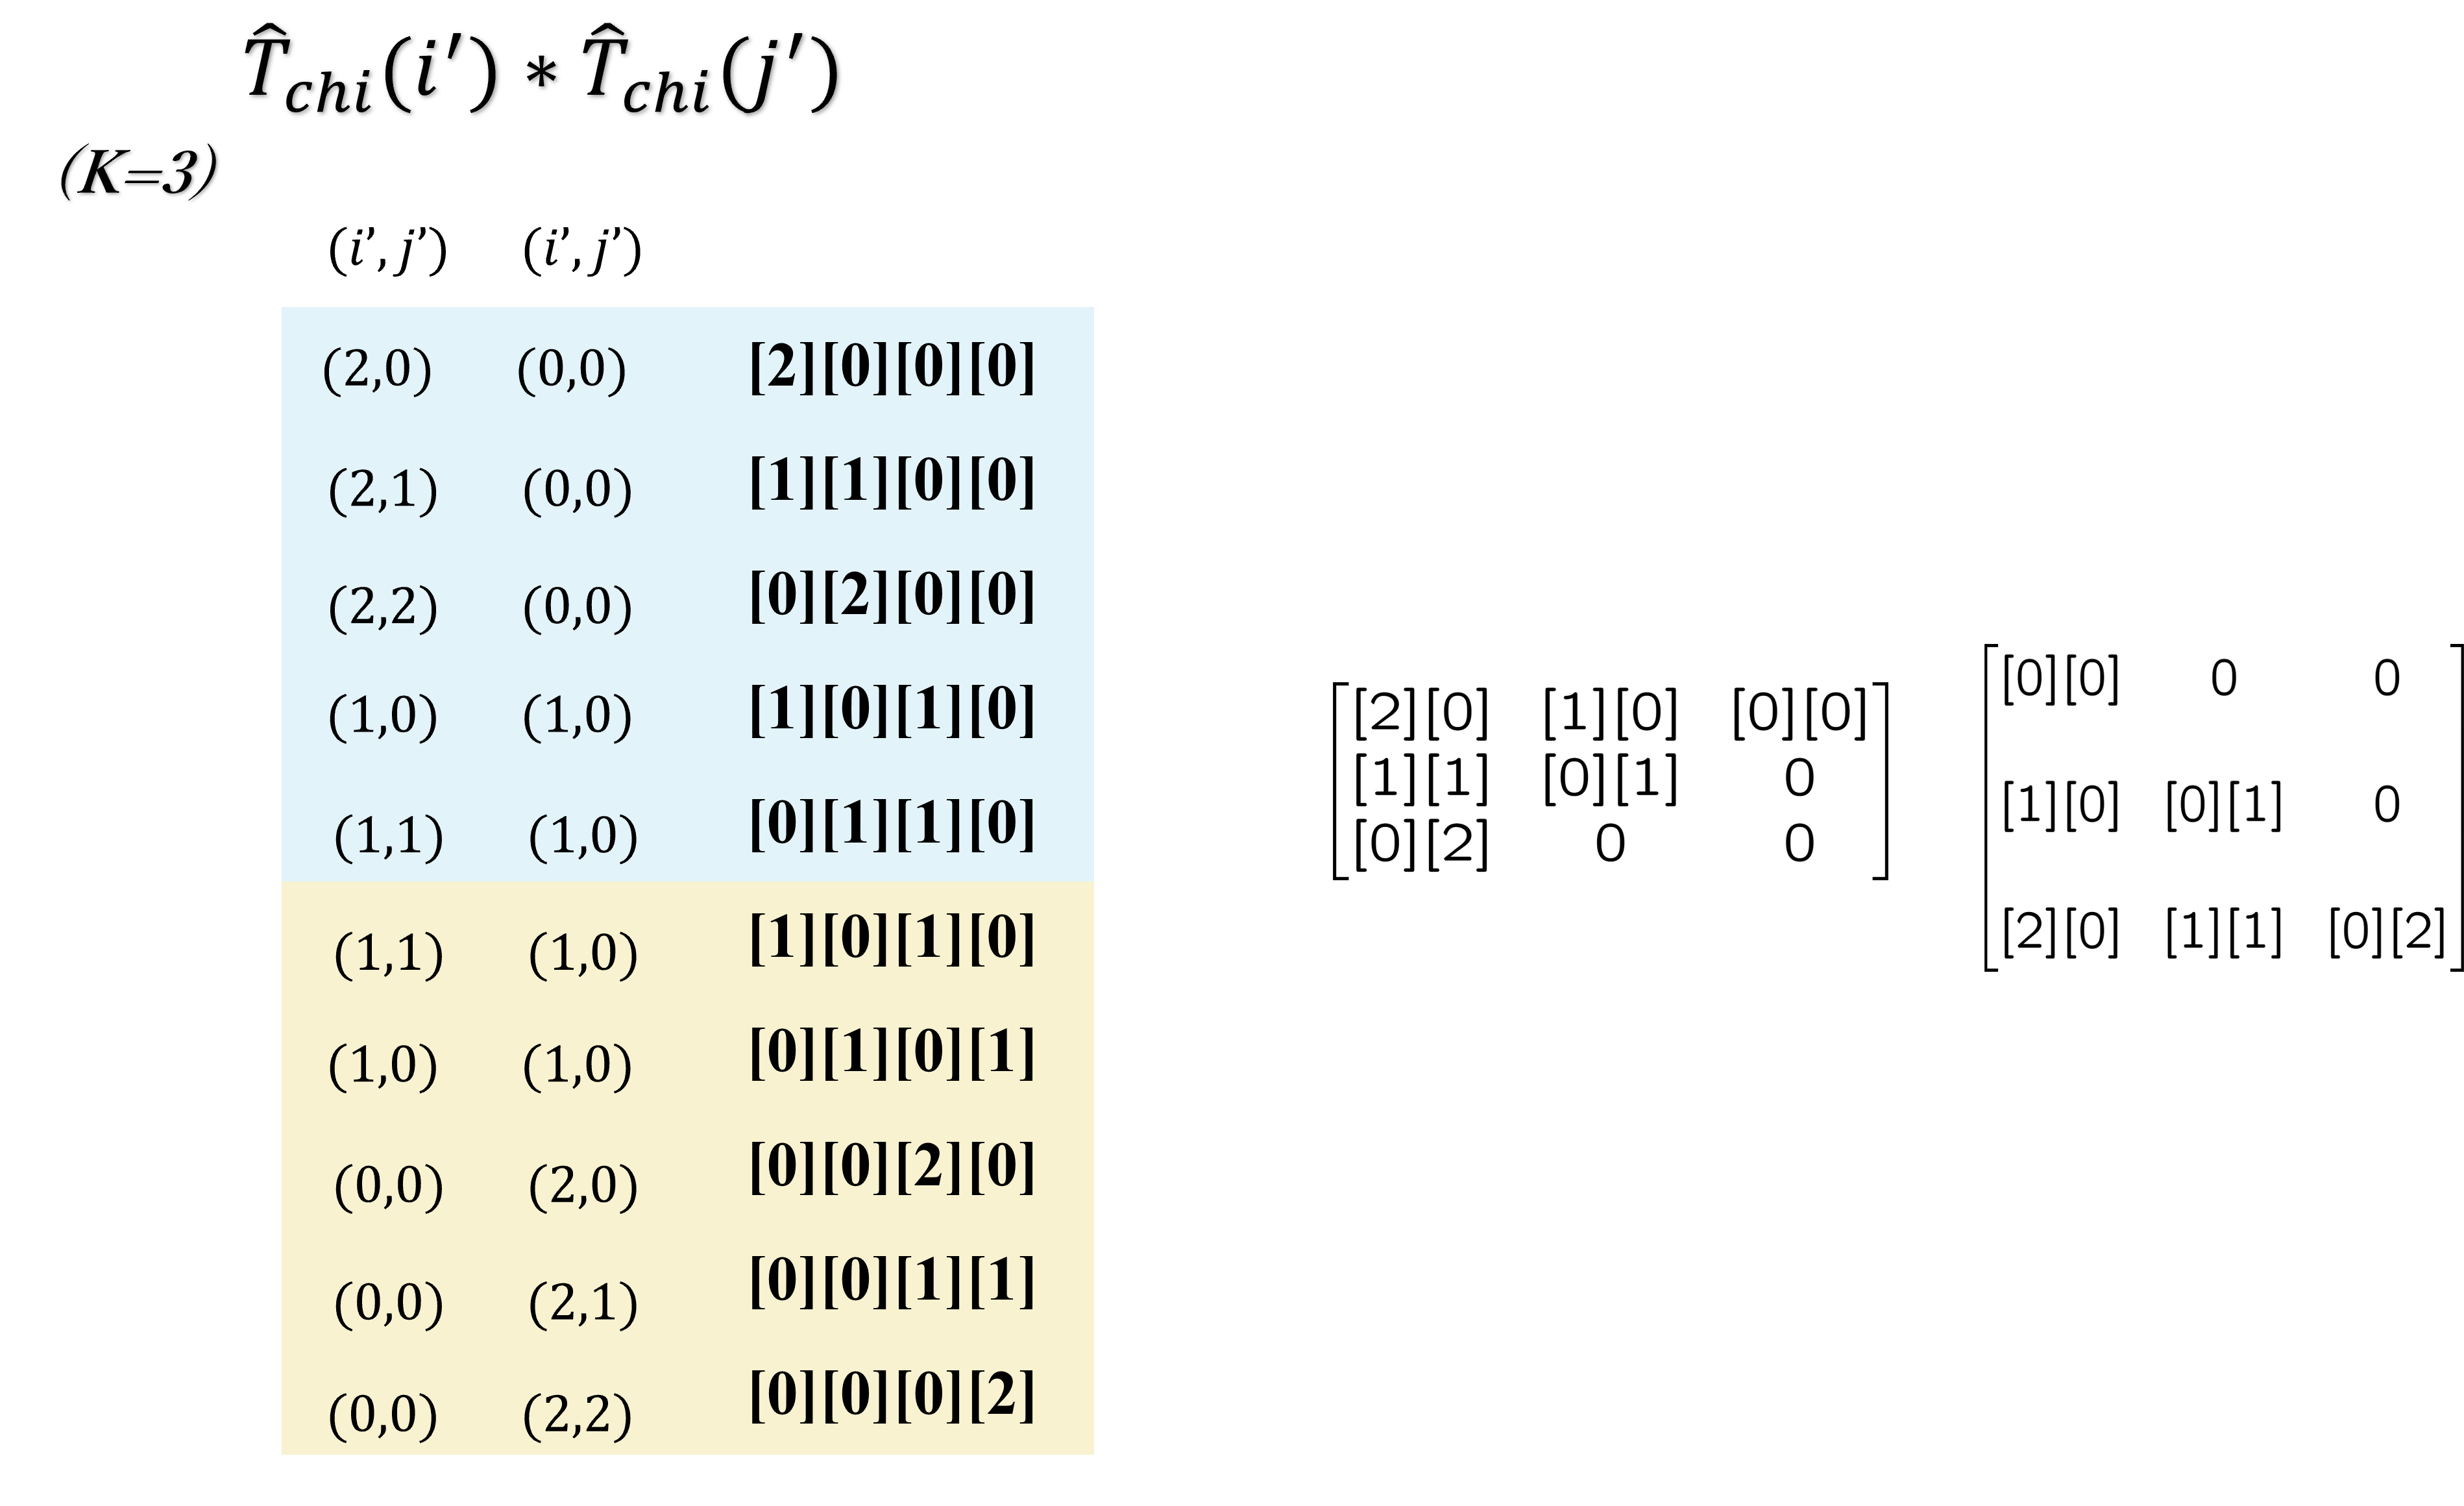
\includegraphics[width=12cm]{TexFigure/Tmat3.png}}
  \caption{Calculation using correlation-matrix}
\end{figure}

\pagebreak

\end{spacing}
\end{document}